\documentclass[11pt]{article}
\usepackage{graphicx}
\usepackage[utf8]{inputenc}
\usepackage{epsfig}
\usepackage{float,graphicx}
\usepackage{listings}
\usepackage{xcolor}
\usepackage{hyperref}
\usepackage{amssymb}
\usepackage{amsmath}
\usepackage{pdfpages}
\usepackage{indentfirst}
\usepackage[margin = 1in]{geometry}

\definecolor{codegreen}{rgb}{0,0.6,0}
\definecolor{codegray}{rgb}{0.5,0.5,0.5}
\definecolor{codepurple}{rgb}{0,0,0}
\definecolor{backcolour}{rgb}{1,1,1}

\hypersetup{
 colorlinks,
 citecolor=blue,
 linkcolor=blue,
 urlcolor=blue}

\lstdefinestyle{mystyle}{
    backgroundcolor=\color{backcolour},
    commentstyle=\color{codegreen},
    keywordstyle=\color{black},
    numberstyle=\tiny\color{codegray},
    stringstyle=\color{codepurple},
    basicstyle=\ttfamily\footnotesize,
    breakatwhitespace=false,
    breaklines=true,
    captionpos=b,
    keepspaces=true,
    numbers=left,
    numbersep=5pt,
    showspaces=false,
    showstringspaces=false,
    showtabs=false,
    tabsize=2
}

\lstset{style=mystyle}
\title{Summer of Science 2023\\
\textbf{Criminology: Mid-Term Report}}

\author{Yash Paritkar\\
Roll Number: 210070096\\
\\
Mentor: Dev Pratap}

\date{May-July 2023}

\begin{document}

\maketitle

\newpage

\begin{abstract}
    This mid-term report aims to highlight the basics of the theory of criminology. The learning so far covers the basics of criminology and classical criminology concepts. This project starts with a definition of crime and various types of crime and then moves on to the different theories that try to explain why individuals commit crimes or why all people do not commit crimes. The learning is done solely from the book Introduction to Criminology by Hassan et al. \cite{ref: Introduction to Criminology}. As the authors of the book are Canadian, the book focuses more on the scene in the Canada.
\end{abstract}

\tableofcontents

\newpage

\section{What is Crime?}

\subsection{Introduction to Crime}
The word crime derives its roots from the Latin word crimen. Hence, criminology is the study of crime. It is the discipline that takes crime as its object of study, first emerged within Europe in the late 19th century. Cesare Lombroso is referred to as the "father of criminology".

Early criminologists believed crime was something rooted in our evolution or, more specifically, in the failure of criminals to develop adaptive traits like empathy and honesty. It was French sociologist Émile Durkheim who started the course of modern criminology. He stated

\begin{itemize}
    \item crime in fact is a normal part of every society and something that can never really be eliminated
    \item crime performs an important function for society in that it establishes the norms for what is acceptable behaviour.
    \item “offends certain collective feelings which are especially strong”
\end{itemize}

As criminology initially considered crimes against the state, it was obvious for the criminologists to see indigenous people through the lens of racism. These also led to modern criminology being oriented more towards retribution rather than restitution, like indigenous justice systems.

\subsection{Crime in Canada}

Crimes are transgressions that violate the laws a society holds dear. These laws may be formally written down, held by knowledge keepers, or commonly known to all members of the group. To commit a crime is to break the rules a society views as the moral limits of acceptable behaviour.

There are two important terms in crime:

\begin{itemize}
    \item 	\textit{actus reus}: a person must have committed a guilty act
    \item 	\textit{mens rea}: guilty frame of mind at the time of offence
\end{itemize}

There are a few main approaches to crime, one of which is the legalistic approach. In a legalistic approach, crime is mainly seen in relation to Criminal Code. In Canadian Criminal Law, a person may be charged with two main types of criminal offences: summary and indictable.

Codified laws are important in understanding what crime is. The initial usage of them can  be found as far back as 4000 years ago, with the codes of Ur-Nammu and Hammurabi. They provide an objective and statistical approach to the crime. Although many criminologists find this approach problematic as Law is a historical and cultural product, i.e. a social construct.

Some laws do emerge from consensus, but many laws serve the purpose of the ruling class in dominant over the other folks. This is especially important in corporate crimes.

\subsection{Colonialism as Crime}
Nielsen and Robyn (2019) explain that “colonialism is a classic state crime that relies on violence and the threat of violence to achieve political and economics ends”. Viewing colonialism as a crime is not simply about recognising that the land was stolen and the original inhabitants harmed; it is about the law’s power to define who is to be considered a worthy victim (Christie, 1986) and who can get away with murder. Law is an arena of conflict that determines who is a criminal.

\subsection{Framing Crime}

The media effectively amplifies particular threats, sometimes to the point of generating moral panics and constructing representations of groups (e.g., youth, the working class, and racialised communities) as posing a threat to public well-being. Hence, media is a powerful instrument in understanding crime.

\section{Typologies and Patterns of Crime}


\subsection{Introduction: Thinking Critically about Crime}

Voting, political action, cultural practices, and media debates—society collectively decides which types of behaviour are considered harmful or criminal. We have consensus on this. Consensus is a general agreement. e.g., murder is crime.

Not all the crimes have consensus. What is crime is also decided by governing body which is many times composod of dominant groups such as colonisers. Indigenous peoples are overrepresented in the criminal justice system as both victims and offenders (Monchalin, 2016) and also receive harsher sentences. The overrepresentation of Indigenous peoples in criminal justice statistics is connected to a history of criminalising Indigenous culture.

\subsection{Thinking about Crime: Classification and Typologies}

Some criminologists suggest that we view crime as a violation of conduct norms. Deviance refers to behaviours that depart from or violates social norms.

Typology is special system of classifying different types of crime. One of the simplest one is violent crime, property crime, other crime, traffic offences, federal drug offences, and other federal law violations. Another common approach is divide criminal acts into victimless crimes (e.g., drug use, prostitution, and illegal gambling) and crimes where there is a clear victim (e.g., robberies and physical assaults). One more obvious type is to divide into street crime and white coller crimes.

The book does the following classification into 6 categories, namely violent crime, property crime, organised crime, hate crime and terrorism, white collered crime and corporate crime.

\begin{itemize}
    \item \textbf{Violent crime}:This includes homicide (delibrate and unlawful killing of the one person by another), assault (to injure somebody seriously, causing permanent damage to their body), sexual assault and robbery (use of violence while commiting theft).

    \item \textbf{Non-Violent Crimes}:This includes breaking and entering (generally done on property owned by the upper middle class people), theft and identity theft.

    \item \textbf{Crimes of Morality and Public Order}:This includes crime which are disregarded for the society as a whole on moral basis for example prostitution and drug use.
    
    \item \textbf{organised Crime}: They are most commonly involved in drug and gun trafficking; however, human trafficking and computer-based crime have become increasingly common amongst these groups. These groups have high level of internal structure.
    
    \item \textbf{Hate Crime,Extremism and Terrorism}: Hate crimes are statements which can be aggravating factor that precede violence
    
\end{itemize}

\subsection{Crime Patterns Over Time}

Initially crime rate started increasing with increase in population but due to internet age, the figure is going down. The dark figure of crime i.e. unreported crime is also increasing for example, why would one steal CD from Walmart if he could download song from internet.

The COVID-19 pandemic and subsequent lockdown is the largest criminological experiment in the history. It altered the crime patterns.

\section{Media and Crime}

Although media may not offer a thorough or accurate depiction of crime and justice (as is discussed in this chapter), it is important to examine the ideas and images they produce. The  image \ref{Newsworthy} shows a rough noteworthiness criteris.

\begin{figure}
    \begin{center}
        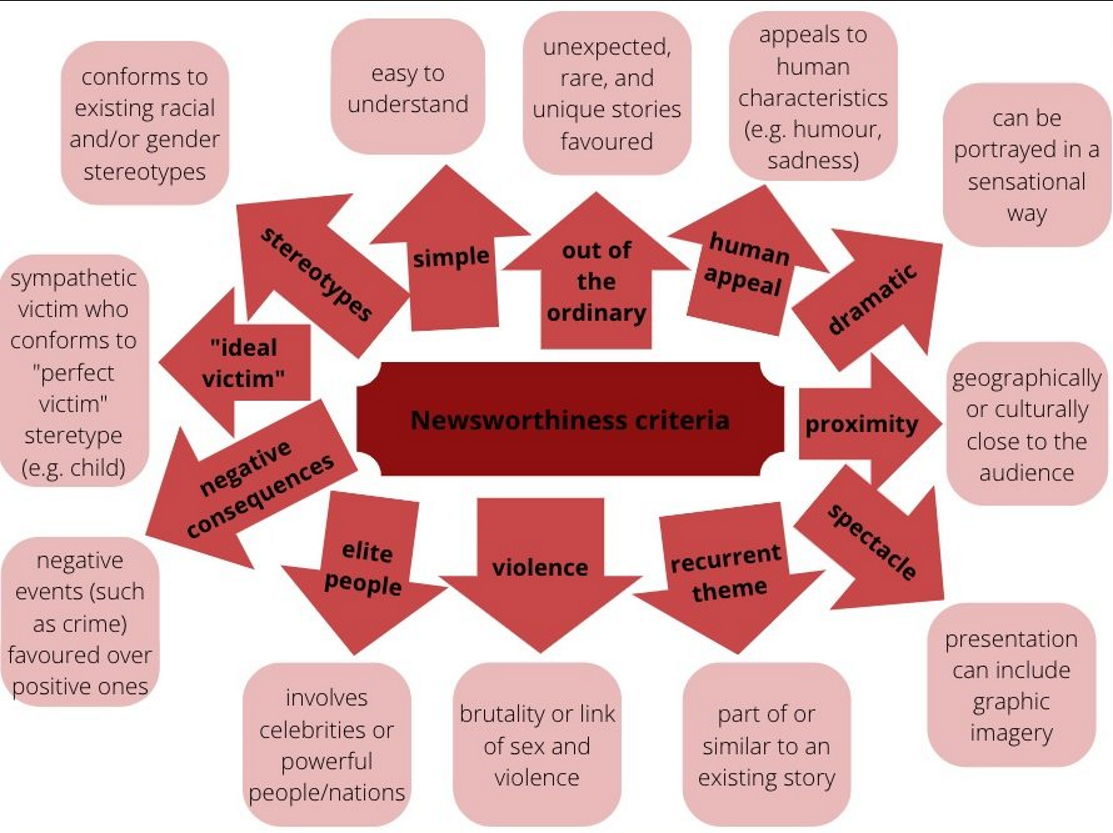
\includegraphics[width = 4in]{Newsworthy.png}
    \end{center}
    \caption{Newsworthiness criteria \cite{ref: Newsworthiness Criteria Image}}
    \label{Newsworthy}
\end{figure}

\subsection{Theoretical Perspectives on the Relationship Between Crime, Media and the Public}

Due to obvious reasons, the media cannot show the whole picture. Hence the question arises, who decides which stories to tell and how to tell them?

There are several models which discuss which story to show or are shown.

\begin{itemize}
    \item Market Model: Media is a business and crime news is a product that meets market. There is no need to regulate the market.
    
    \item Social Responsibility Model: Media is a tool for developing an informed citizenry and media requires regulation.
    
    \item Propaganda Model: Media contents represent the itnerests of the powerful and street crimes serves to divert attention.
    
    \item Organizational Model: Content of news is dictated by the routines of news production and reliance on established sources and story lines.
    
    \item Cultural Studies Model: Media content is a cultural product that serves to socially construct meaning and media representation may produce and reproduce social constructions and may be contested
\end{itemize}

\subsection{How Media Frame Portrayals of Offenders, Victims, and Police}

Frame sets limits of what you can see, similar thing happen to media framing. It is done using images, positioning of the content on the news paper and using stylised, bold/italic fonts.

The rarest crimes receive the most coverage, while the most common crimes rarely receive coverage. \textbf{Racialisation of crime} is also prevelant, that is people from vlnurable (racial, castist or female) are blamed for being both victim and offender. Media also tend to portray gangs as highly organised. Views which differ from enforcements have hard time to get coverage in the media.

New media shift the role of the audience from passive consumers to active participants. Looping” between the legacy and new media is apparent. Looping refers to the recycling of media content in different formats, different contexts, and different outlets.

\section{Race and Crime}

\subsection{The Origins of Race and Racism}

Race is a social invention, also referred to as a social construct that is, in part, a historical product of Western European colonization and the systems of Trans-Atlantic slavery.
A critical perspective on race is that, race is artificial social construct and not a natural category.

\subsection{Colonialism and Criminal Justice}

\textbf{Colonialism} often refers to how European expansionism moved throughout the world beginning in the 15th century. And with the introduction of European logic, science, rule of law, government, trade and religion, the locals are termed as savages. Colonization is the implementation of a political, legal, and economic system that is controlled through a foreign sovereign authority.

Europeans also follow \textbf{Doctrine of Discovery}, that is god has given right to conquer and colonize lands earlier inhibited by christins.

\subsection{The Practices of Race in Colonialism}

Scholars argue that colonialism is a system of governance that relies upon institutional forms of racism that develop over three stages

\begin{itemize}
    \item First, invent disctinction to separate themselves between the population to be controlled
    
    \item Second, try to justify control by using idea that colonised people are different type of humans
    
    \item Thirdly, understand yourselves as superiors
\end{itemize}

This results in \textit{kill the Indian in him, and save the man}. Today, the race as an action is an act that is “done” to someone in that people or subjects can be “racialised” by a person, an act, or a system.

\subsection{Police Racial Profiling}

Racial profiling is the use of race by police and border security to select subjects for surveillance, detention, and/or arrest. A common problem with studies of racial profiling is that the research seldom differentiates between different racial minorities.

\subsection{Intersectionality}

Intersectionality is an analytical framework for understanding how a person's various social and political identities combine to create different modes of discrimination and privilege. Intersectionality identifies multiple factors of advantage and disadvantage. Practise of racism can be divided into three categories on the bases if how they are deployed in real practice:

\begin{itemize}
    \item Overt Racism: It is kind of racism individuals experience as direct interpersonal experiences.
    
    \item Institutional Racism: Racism without racists.
    
    \item Systemic Racism: Bias or difference experienced as an 
    effect of the of social structures.
\end{itemize}

\section{Methods and Counting Crime}

\subsection{The Research Process}

An understanding of quality research methods is fundamental to informed citizenship, scientific advancement, economic activity and government decision-making. This is true for criminology also. The research process is consists of 9 steps:

\begin{enumerate}
    \item Planning
    \item Conceptualization
    \item Choice of Method
    \item Operationalization
    \item Sampling
    \item Data Collection
    \item Data Planning
    \item Analysis
    \item Application
\end{enumerate}

Most Western researchers follow the Newtonian epistemology that “scientific knowledge has to provide an objective representation of the external world,”. This ignores the connection between factors. One method more suited to criminology while data collection is talking circle in which all members of the group sit in the circle, one has a stone, only he can speak, he will pass after his talk is finished.

\subsection{Use of Research Findings}

Harm can come from how results are shared with others. For instance, if a researcher states that there are higher rates of financial exploitation in a certain Indigenous community than in the broader society, this implies that the tribal people tend to be more criminal, creating a negative stereotype. This kind of ill conclusions can cause a great harm to section of people since crime are involved.

\section{Biological Influences on Criminal Behaviour}

Biological theories allow criminologists to differentiate between the effects of environment, lived experiences, and genotype on antisocial behaviour and understand how the two interact to evaluate the impact of stress on the epigenome.In the past, many people started believing that all behaviour was based on biological traits with no room for environmental impact.

Phrenology, a theory of human behavior based upon the belief that an individual’s character and mental faculties correlate with the shape of their head, was one of the earliest biological theories of crime and laid the foundation for the development of the biological school of criminology. Franz Gall was one of the early proponents of phrenology. Biological positivism and determinism was also prevelant. All of this along with eugenics specially negative eugenics and pseudoscience led to holocaust.

\subsection{Genetics}

A common misconception is that  the link between biology and crime is primarily genetic. Most behaviours are not criminogenic on their own, but under the right circumstances could lead to a person offending. Eg, impulsivity.As with all studies of genetics, twins offer a great opportunity to study the effect of genetics on crime. Although, adoption gives a better way to study the effect of genetics in criminology as adoption provides the same environment but different genetic composition.

Person with certain genetic backgrounds are more sensitive to specific environmental triggers than others. Someone without a predisposition for criminal behaviour may never offend, irrespective of an adverse environment, and a person with a predisposition for criminal behaviour may never offend if they do not experience adversity.

The genome of person great number of genes, which may or may not be expressed and can also be in varying amounts. This is called epigenetics. Epigenetic studies help us understand why atrocities such as residential schools not only had major and long-lasting impacts on the Indigenous children who were abused, but also how the effect of this abuse is magnified as it is perpetuated biologically through the next generations.

\subsection{Brain Chemistry}

Brain has many neurotransmitters whose concentration affect our  behaviour and their concentration is affected by both genome and environment. Few neurotransmitters like serotonin, dopamine and monoamine oxidase (MAO) has significant impact on functioning of brain and hence are abused as drugs by many.

\subsection{Brain Damage and Disorders}
The frontal lobe, found from the forehead region above the eyes to the midway of the skull, is heavily involved in inhibiting inappropriate behaviour, aggression and impulsivity. This area is at the front of the head, so it is more likely to be injured in an accident or assault. Patients lose their social graces, self-control, and patience and may experience personality changes, develop anxiety or depression, demand instant gratification, or have poor planning skills. With a weak skull, children are highly susceptible to frontal brain damage.

Disease and toxins also cause damage to the brain, for example, stroke, brain tumours, meningitis, alcoholism, and cannabis. A patient with a tumour had developed a habit of sexual assault, which was stopped after the tumour was removed, but the habit returned along with the return of the tumour.

\subsection{Nutrition and Alcohol}

Neurotransmitters come from diet. Supplementary diets have shown to have massive improvements in behaviour. Foetal Alcohol Syndrome (FAS), which occurs due to prenatal alcohol consumption have serious effects on the developing brain of foetus. This result in children developing cognition, attention, communication, and perceptual deficits; hyperactivity; an inability to understand consequences; and poor peer relationships.

\section{Psychological Theories of Crime}

Psychology aims to answer the question, "Why do people break the law?". This is done via both individual approach and social approach. 

\subsubsection*{Nurture}

Research on children has shown that behaviour/temperament developed in the first three years of life is carried forward in the life. For a criminal those are high sensation seeking  combined with low self-control and negative emotionality combined with callous emotional trait. One of the most famous personality type classification is Myers-Brigg:
\begin{itemize}
    \item E/I: Extraversion or Introversion
    \item S/N: Sensing or Thinking
    \item T/F: Thinking or Feeling
    \item J/P: Judging or Perceiving
\end{itemize}

\subsubsection*{Nurture}

Argues that personality develops in response to childhood experiences. Freud proposed five stages of psychosexual development. According to him, human is sexual being and sexualness is expressed in different ways on different age. Erik Erikson expanded this theory throughout life span. At each stage of life, individuals face developmental challenges on the road to self-actualisation. Theories proposed by Baumrind (parenting style),Patterson (coercion theory) and Bowlby (attachment theory) use parenting style to describe behavior of children.

\subsection{Cognitive \& Cognitive-Behavioural Theories of Criminal Behaviour}

These look for faults in cognitive processes, mental development and/or a defective moral compass. These look at the way thoughts and feelings influence human behaviour. 	• The cognitive aspect of cognitive-behavioural psychology examines how reinforcement and punishment turn into thoughts, beliefs, and attitudes that maintain and justify behaviour. Bonta and Andrews (2017) summarise key links between antisocial attitudes and antisocial behaviour.

Heuristics are mental shortcuts that allow us to filter and process the massive amount of information we are faced with on a daily basis. They are necessary to make decisions but they are affected by cognitive bias.
\begin{itemize}
    \item Confirmation bias: Tendency to over-value evidence that confirms our beliefs over evidence that counters our belief
	
    \item In-group bias: Tendency to trust peers and colleagues more than those outside your group
\end{itemize}

\subsection{Medical Model of Psychology and Criminal Behaviour}

Mental illness would seem to fall solidly in the camp of individual psychology, the interface between mental illness and criminality is as much socially determined as it is individually determined. There are few "illnesses" which result in criminological behavior
\begin{itemize}
    \item Antisocial Personality Disorder: persistent, longstanding, maladaptive ways of thinking and feeling about oneself and others that detrimentally affect how one functions. Strongly linked with violence.
    
    \item Psychopathy: Interpersonal and emotional traits, such as manipulation, grandiosity and impaired empathy. Antisocial behaviour and lifestyle traits, such as impulsive behaviour sensation seeking and a parasitic lifestyle.
    
    \item Psychosis: Psychosis is a condition that impacts how your brain processes information and is present in some severe mental illnesses, including schizophrenia and mood disorders such as depression and bipolar disorder.
    
    \item  Substance Abuse Disorder: Characterised by difficulties reducing substance use. It has three part (Tripartite concept model by Goldstein), systemic crime, economically compulsive crimes and psychopharmacologically-driven crime. Delegalizing them involves increasing profit and thereby risk taking abilities of suppliers including violence. A notable example is of Portugal's war on drugs
\end{itemize}

\subsection{Trauma-Informed Neurobiology and Criminal Behaviour}
\subsubsection*{Adverse Childhood Experiences(ACE)}

ACEs have been linked to cause of death. Toxic Stress is prolonged activation of stress response systems in the absence of protective relationships. 	• Toxic stress causes the amygdala to get inflamed and hippocampus to lose volume. The individual experiences poor impulse control, challenges with deciphering when real danger is truly present, and a quickly activated fight/flight stress response system. However, this mechanism is not useful in daily life. Children facing domestic abuse in young age gets his sympathetic nervous system triggered too often.

\subsubsection*{Trauma-Informed Models of Addiction}

The trauma-informed model of addiction acknowledges a physiological, brain-based vulnerability to addiction that is influenced by genetics but also heavily impacted by supports and positive or negative experiences/influences in one’s life.

Post-traumatic stress disorder (PTSD) is caused by traumatic life events, resulting in persistent re-experiencing of the event; avoidance of feelings, thoughts, conversations or places associated with the trauma; adverse alterations in cognition and mood; and hyper-arousal. PTSD is assiciated with substance abuse.

\subsection{Evolutionary Psychology}

Evolutionary psychology posits that the ultimate function of all biological organisms is to increase their reproductive success. It looks at unconscious psychological mechanisms that would've been adaptive in the environment in which they evolved. Social mores change much more rapidly than genomes. It explains why age-crime curves aligns with sexual maturity curve

\subsection{Cultural Psychology}

It look at how individual behaviour is constructed by society. Subcultures can create norms that contradicts those of the society in which one lives in. Tough on crime policies are less effective than intervention, prevention and rehab approach.

Restorative Justice: theory of justice that focuses on the harm caused by crime and wrongdoing to people, relationships and community. It provides a framework for addressing and preventing harm that moves beyond punishment towards healing. There is need for public ceremonies or recognition of rehab. Conviction and incarceration are often highly public acts while rehab is completely private process

\subsection{Integrative Models of Criminality}
4 Models that integrate theories from individual, evolutionary and cultural approaches

\begin{itemize}
    \item Moffitt’s Developmental Taxonomy: explains the development of antisocial behaviour as affected by biology, socialisation, and stages of development. 
    \item General Aggression Model: explains the biological, personality, cognitive and social learning factors influencing an aggressive act. 
    \item Risk Needs Responsivity Model: provides a method for offender assessment and treatment by examining the needs underlying criminal behaviour. 
    \item Trauma-informed Systems of Care: combines the neurobiology of trauma with an analysis of the trauma-inducing aspects of the criminal justice system.
\end{itemize}

\section{Sociological Theories of Crime}

Sociological theories of crime help us understand why some drug use is stigmatised while other use is not, why crime is over- and under-represented across social groups, and what alternatives may exist to the individualistic punishment models that have dominated the criminal justice system since the 19th century.

\subsection{Crime and Social Norms}

It is society that determines what is criminal, not our biology or some universal moral standard. While crime is normal, it is not desirable; it is normal because it establishes the moral boundaries of a community. These lead to development of norms. 

\textbf{Anomie}: a lack of social or moral standards

\subsection{The Chicago School}

The Chicago School had a distinctly macro-level ecological approach to studying crime. Certain zones were marked by greater degrees of social disorganisation due to the transitional nature of these areas as new immigrant communities moved in and older ones moved out. Therefore, fast changing demographics is major invitation for crime. Thrasher argues that gangs are located in interstitial areas of the city, the zones between the settled, more organised neighbourhoods. Zones of transition are characterised by higher levels of residential mobility, ethnic heterogeneity, and lower socio-economic status.

\subsection{Strain Theory}

For Merton, anomie is a condition whereby society exerts pressure on the individual to achieve culturally defined goals but does not provide the institutional means to achieve them or devalues the institutional rules in favour of achieving the goals. Merton lays out five "adaptations" or "modes of adjustment" that people use to relate culturally defined goals with institutional rules. This model was specific to NA but as capitalism has spread across the world, the applicability of this model also. Ends justify the means. This theory is less useful for non-utilitarian crime such as breaking windows, spray painting walls with graffiti and shoplifting of small items.

\subsection{Delinquency as a Subculture}

It is developed by Albert Cohen. It tries to explain crimes that are non-utilitarian, malicious and negativistic. Working class are youth are taught democratic value that everyone can become rich but middle class youths achieve recognition for behaving correctly. There is inversion of values:

\begin{itemize}
    \item middle class places value on controlling aggression and respecting property
    \item the culture of the gang legitimates violence and group stealing
\end{itemize}

When theory was proposed, the status of females was closely tied to males in the 1950s, hence, Cohen argues that most female delinquency tends to be “sexual delinquency”. It fails to explain middle class gangs.

\subsection{Social Control Theory}

Developed by Travis Hirschi (1969). He asked, “Why don’t people engage in criminal behaviour in the first place?”. For him, a person's behaviour is controlled by four types of bonds which are attachment, commitment, involvement and belief. It has mixed results.

\subsection{Labelling Theory}

Roots of theory lies in new way of studying social reality known as symbolic interactionism by George Mead. He explains that we construct our social world and our sense of self through the symbols we exchange. Labelling theory was formulated by Howard Becker. In earlier formulation of labelling theory refers to the process wherein a stigmatising a label leads to a person thinking himself as a criminal.

“Social groups create deviance by making the rules whose infraction constitutes deviance, and by applying those rules to particular people and labelling them as outsiders”

\section{Learning Theories}

\subsection{Criminology and Colonialism}

Indigenous peoples have their own ways of responding to wrongdoing. Criminalisation and over-incarceration perpetuate colonial control and maintain the oppression of the Indigenous other.	The main social influences impacting Indigenous peoples’ justice involvement are structural racism, colonialism, and the Canadian state’s complicity in continued suffering.

\subsection{Learning Theories and Crime}

The social nature of our day-to-day lives has direct implications for our understanding of antisocial behaviour. Learning perspectives of crime suggest that we also learn the motivations, rationalizations, and skills of crime, substance use, and other deviant behaviour.

\subsection{Differential Association Theory}

This theory was proposed by Sutherland. Sutherland articulated the following 9 proposals

\begin{enumerate}
    \item Criminal behaviour is learned.
    \item Criminal behaviour is learned in interaction with other persons in process of communication.
    \item The principal part of the learning of criminal behaviour occurs within intimate personal groups. The important and key people in your social life are where such learning processes occur.
    \item When criminal behaviour is learned, the learning includes (a) techniques of committing the crime, which are sometimes very complicated, sometimes very simple; (b) the specific direction of motives, drives, rationalizations, and attitudes.
    \item The specific direction of motives and drives is learned from definitions of the legal codes as favourable or unfavourable
    \item A person becomes delinquent because of an excess of definitions favourable to violation of law over definitions unfavourable to violation of law.
    \item Differential associations may vary in frequency, duration, priority, and intensity.
    \item The process of learning criminal behaviour by association with criminal and anti-criminal patterns involves all of the mechanisms that are involved in any other learning.
    \item While criminal behaviour is an expression of general needs and values, it is not explained by those general needs and values, since non-criminal behaviour is an expression of the same needs and values.
\end{enumerate}

The primary component of the theory is the role of differential association(s). Individuals have a vast array of social contacts and “intimate personal groups” with whom they interact.

\subsection{Social Learning Theory}
By Burgess and Akers. It has four main components:

\begin{enumerate}
    \item Differential Association
    \item Definitions
    \item Differential reinforcements
    \item Imitation
\end{enumerate}

First two components are similar to differential association theory. There are 4 types of reinforcements, positive reinceforcement, positive punishment, negative reinceforcement and negative punishment.

\subsection{Research in Learning Theories}

A meta-analysis, which synthesises all available research on a particular topic and provides an overall estimate of the empirical relationship, conducted by Pratt et al. (2010) indicated that the impact of deviant associations was moderately strong and equally as important as key factors identified by other criminological theories (i.e., self-control). Differential reinforcement had the overall weakest effects in explaining crime.

\begin{figure}
    \begin{center}
        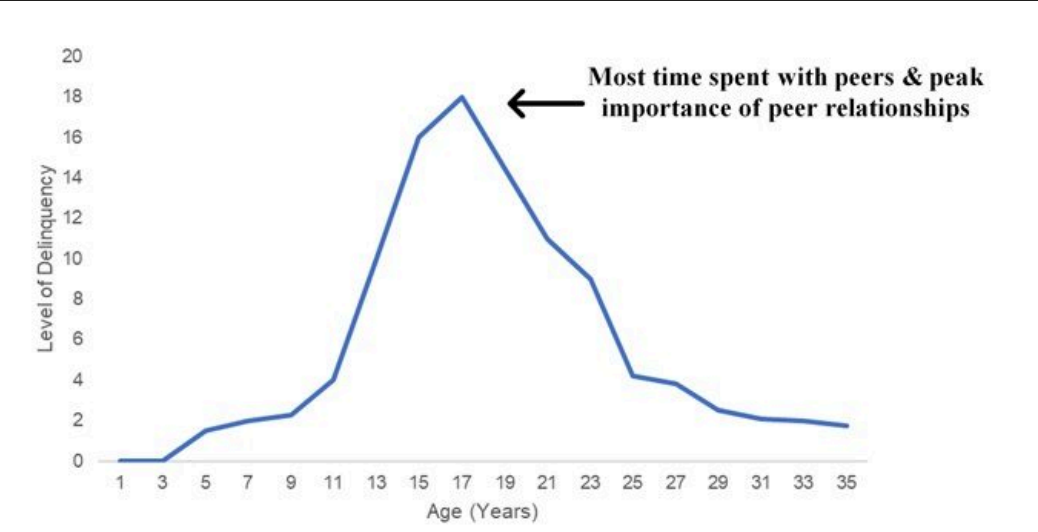
\includegraphics[width = 4in]{Age_Crime.png}
    \end{center}
    \caption{Close relationship between age and crime}
    \label{AgeCrime}
\end{figure}

\begin{itemize}
    \item Age \& Peer: Best known fact in criminology is relationship between age and crime. See image\ref{AgeCrime}
    
    \item Gender \& Peers: Research has suggested that males are exposed to deviant peers more than females. Females spend more time with parents.
    
    \item Turning Points \& Peers: find jobs, get married and possibly serve in the military. The peers at work place disapprove of the crime
\end{itemize}

\subsection{Moving Past a Monolithic Approach to Learning Theory}

Learning theories are often operationalized within western research methodologies. Learning theories do not question the role of the state or include reference to state culpability for human rights violations.

\subsection{A New Approach to Learning Theory}

Peers, friends, romantic partners, and coworkers all have the capacity to inform our attitudes towards deviance and even teach us to commit crime. Learning theories suggest that definitions acquired through associations are important. A potential weakness of social learning theories is the assumption of the universality of mechanisms attached to learning. 


\newpage

\begin{thebibliography}{99}
    \bibitem{ref: Introduction to Criminology}
    {Introduction to Criminology\\
    \url{https://open.umn.edu/opentextbooks/textbooks/1327}}

    \bibitem{ref: Newsworthiness Criteria Image}
    {Newsworthiness Criteria\\
    \url{https://kpu.pressbooks.pub/app/uploads/sites/199/2022/08/Figure-1-red-version-e1661459196776.jpeg}}


\end{thebibliography}

\end{document}